\subsection{Varying Diffusion Coefficients}
For the first set up, the neural network is defined using the Keras API, with an input layer of 2 neurons (corresponding to position and time), two hidden layers of $50$ neurons each, and a linear output layer. The model is compiled with the mean squared error loss function and the RMSprop optimizer with a learning rate of $0.001$. The model is then trained for $200$ epochs on the shuffled training data, with a batch size of $256$ and a validation split of $0.2$. The training loss and validation loss are plotted as a function of the number of epochs. It showed good prediction with minimum loss function shown in Figure (\ref{fig:tls}). This was then followed by a contour plot immediately to test the model.

\begin{figure}[htb!]
% \begin{center}
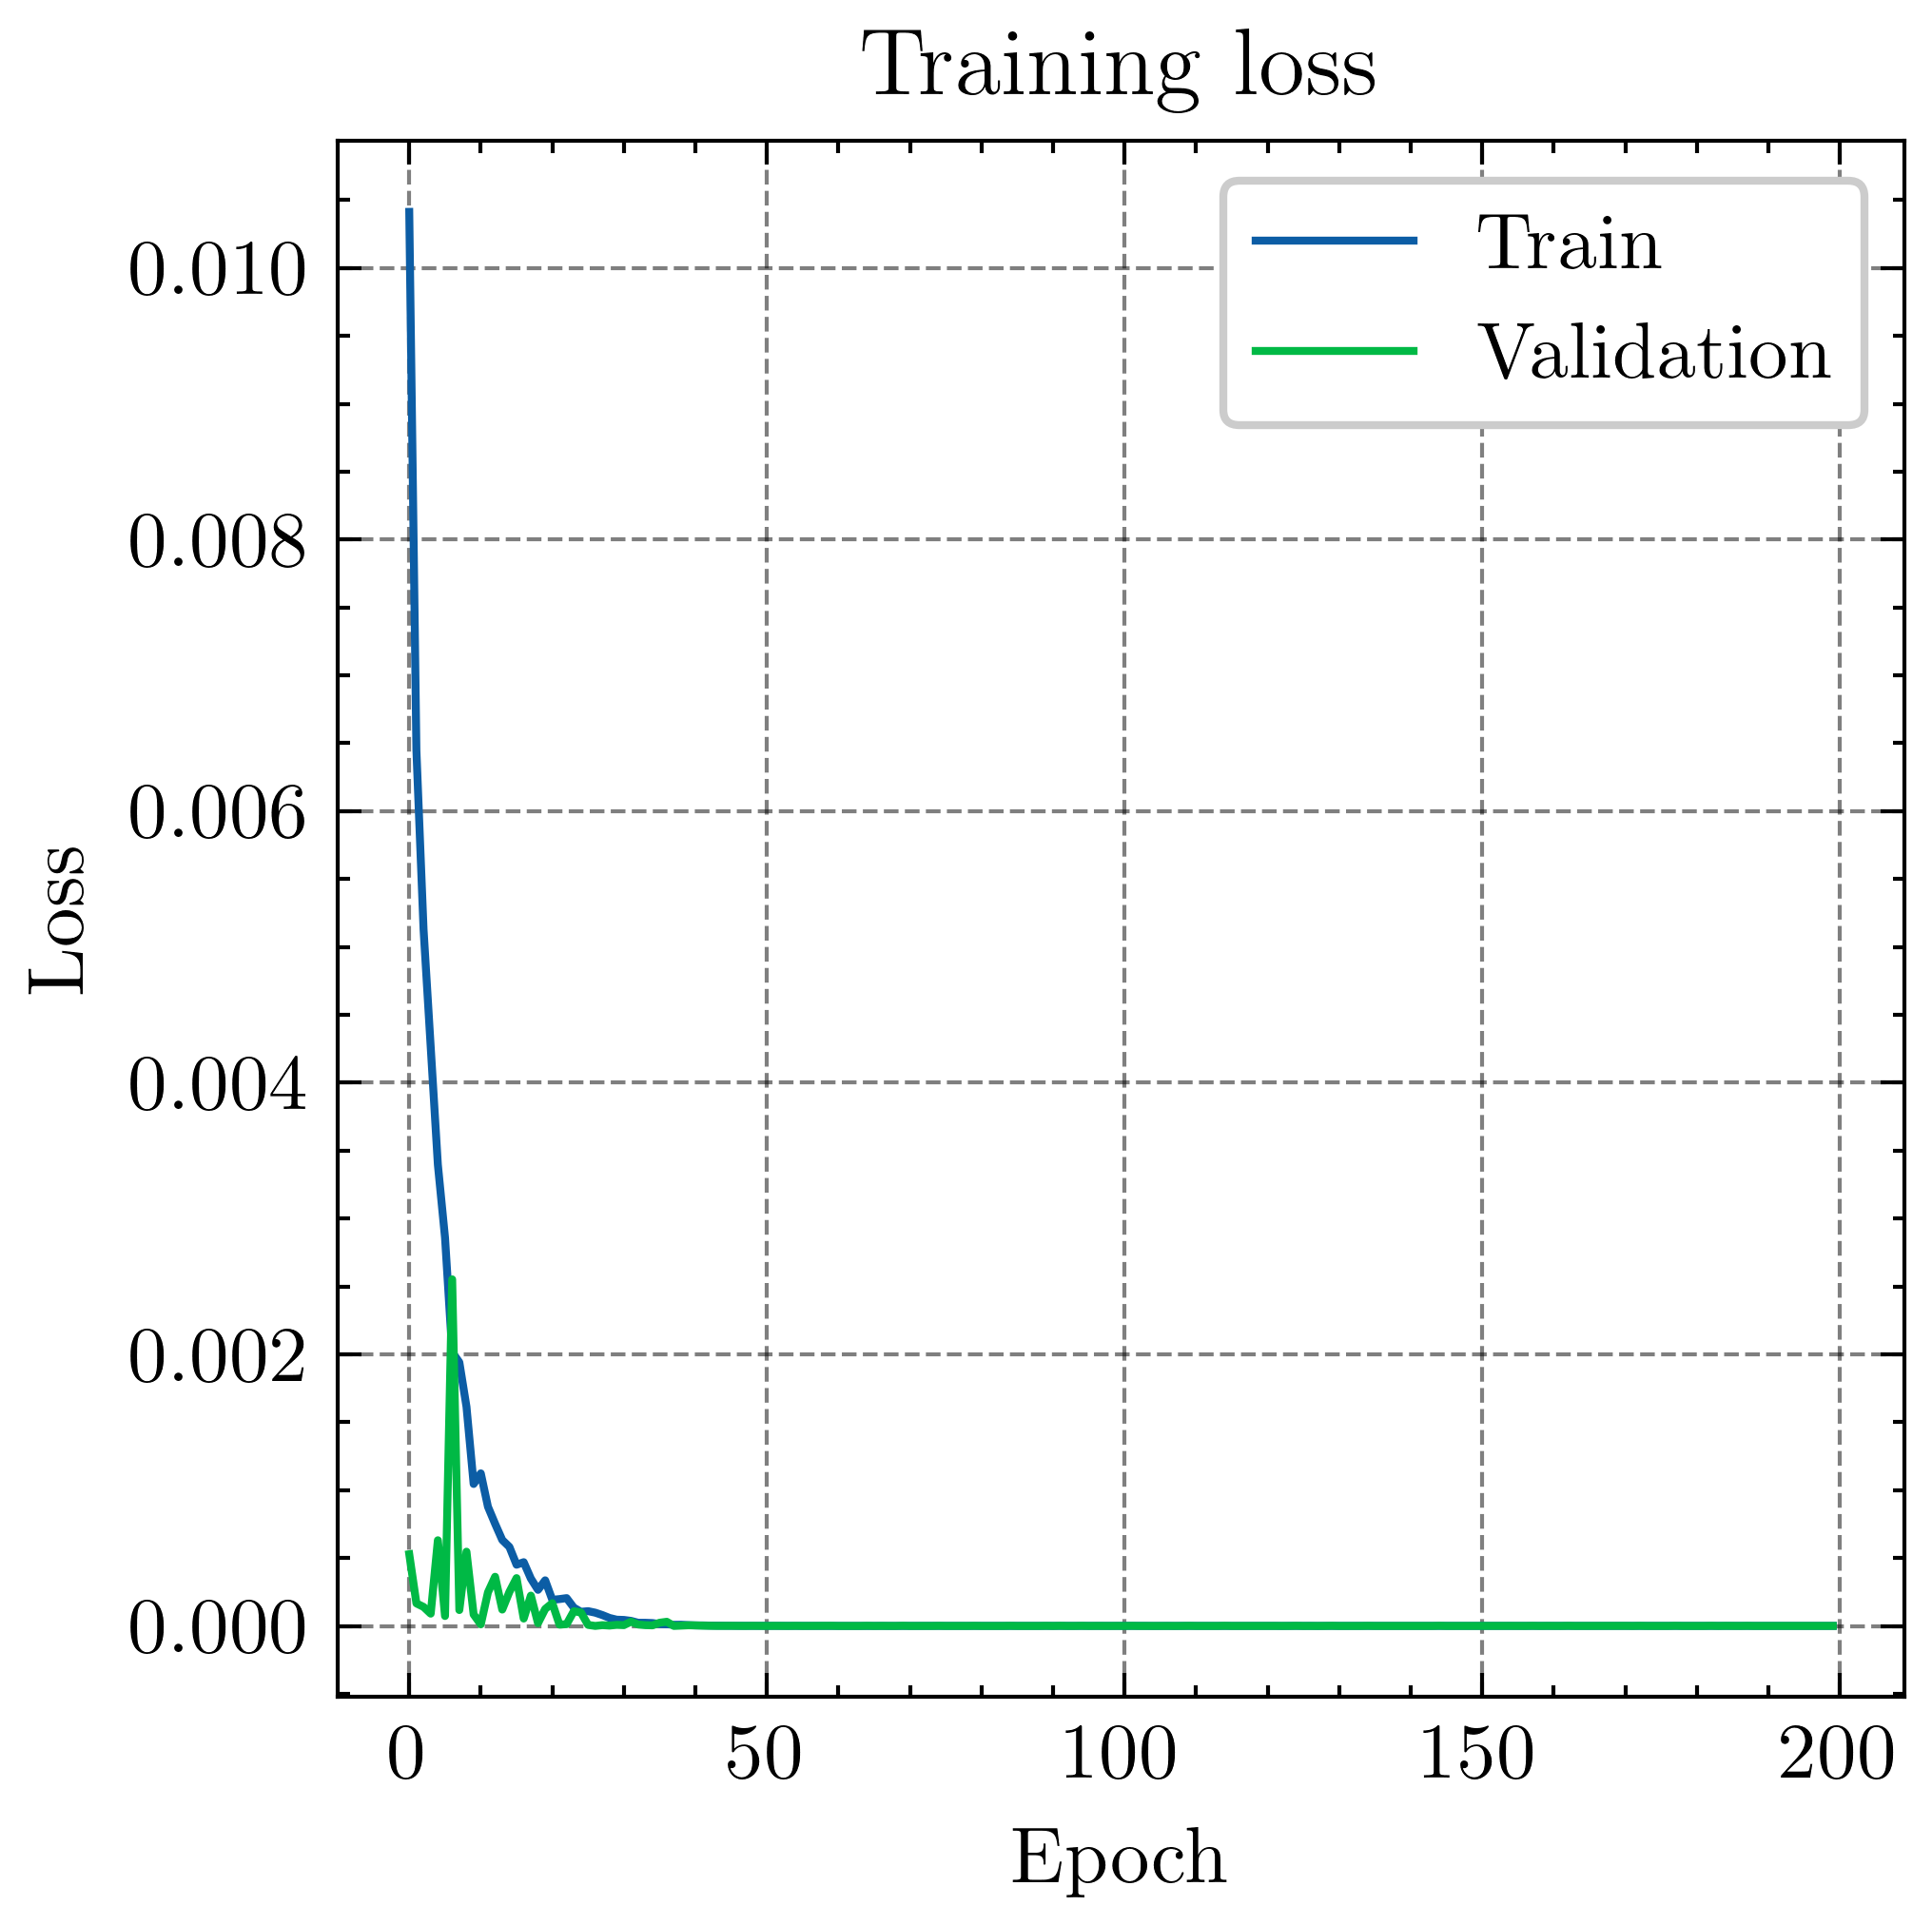
\includegraphics[width=.49\textwidth]{images/train_loss.png}
\vspace*{-8mm}
\caption{Model training and loss, based on the number of $epochs=200$ and $batch\_size=256$. It can be observed that there's nearly no loss of data after the $20^{th}$ epoch}.
\label{fig:tls}
% \end{center}
\end{figure}

The four contour plots in Figure (\ref{fig:alld}) show the predicted solution of the diffusion equation for different values of coefficients $D$ ranging $0.1 , 0.2, 0.3$ and $0.4$. This is done  by evaluating the trained neural network on the entire domain and plotting the results. From the contour plots we can arrive at the conclusion that the predicted values of the diffusion equation are consistent with the expected behavior of diffusion. For example, at early times, the diffusion is localized around the initial position, while at later times, it spreads out and becomes more diffuse. We also see that the diffusion is slower for lower values of the diffusion coefficient, which is consistent with our understanding of diffusion.

\begin{figure}[htb!]
\begin{center}
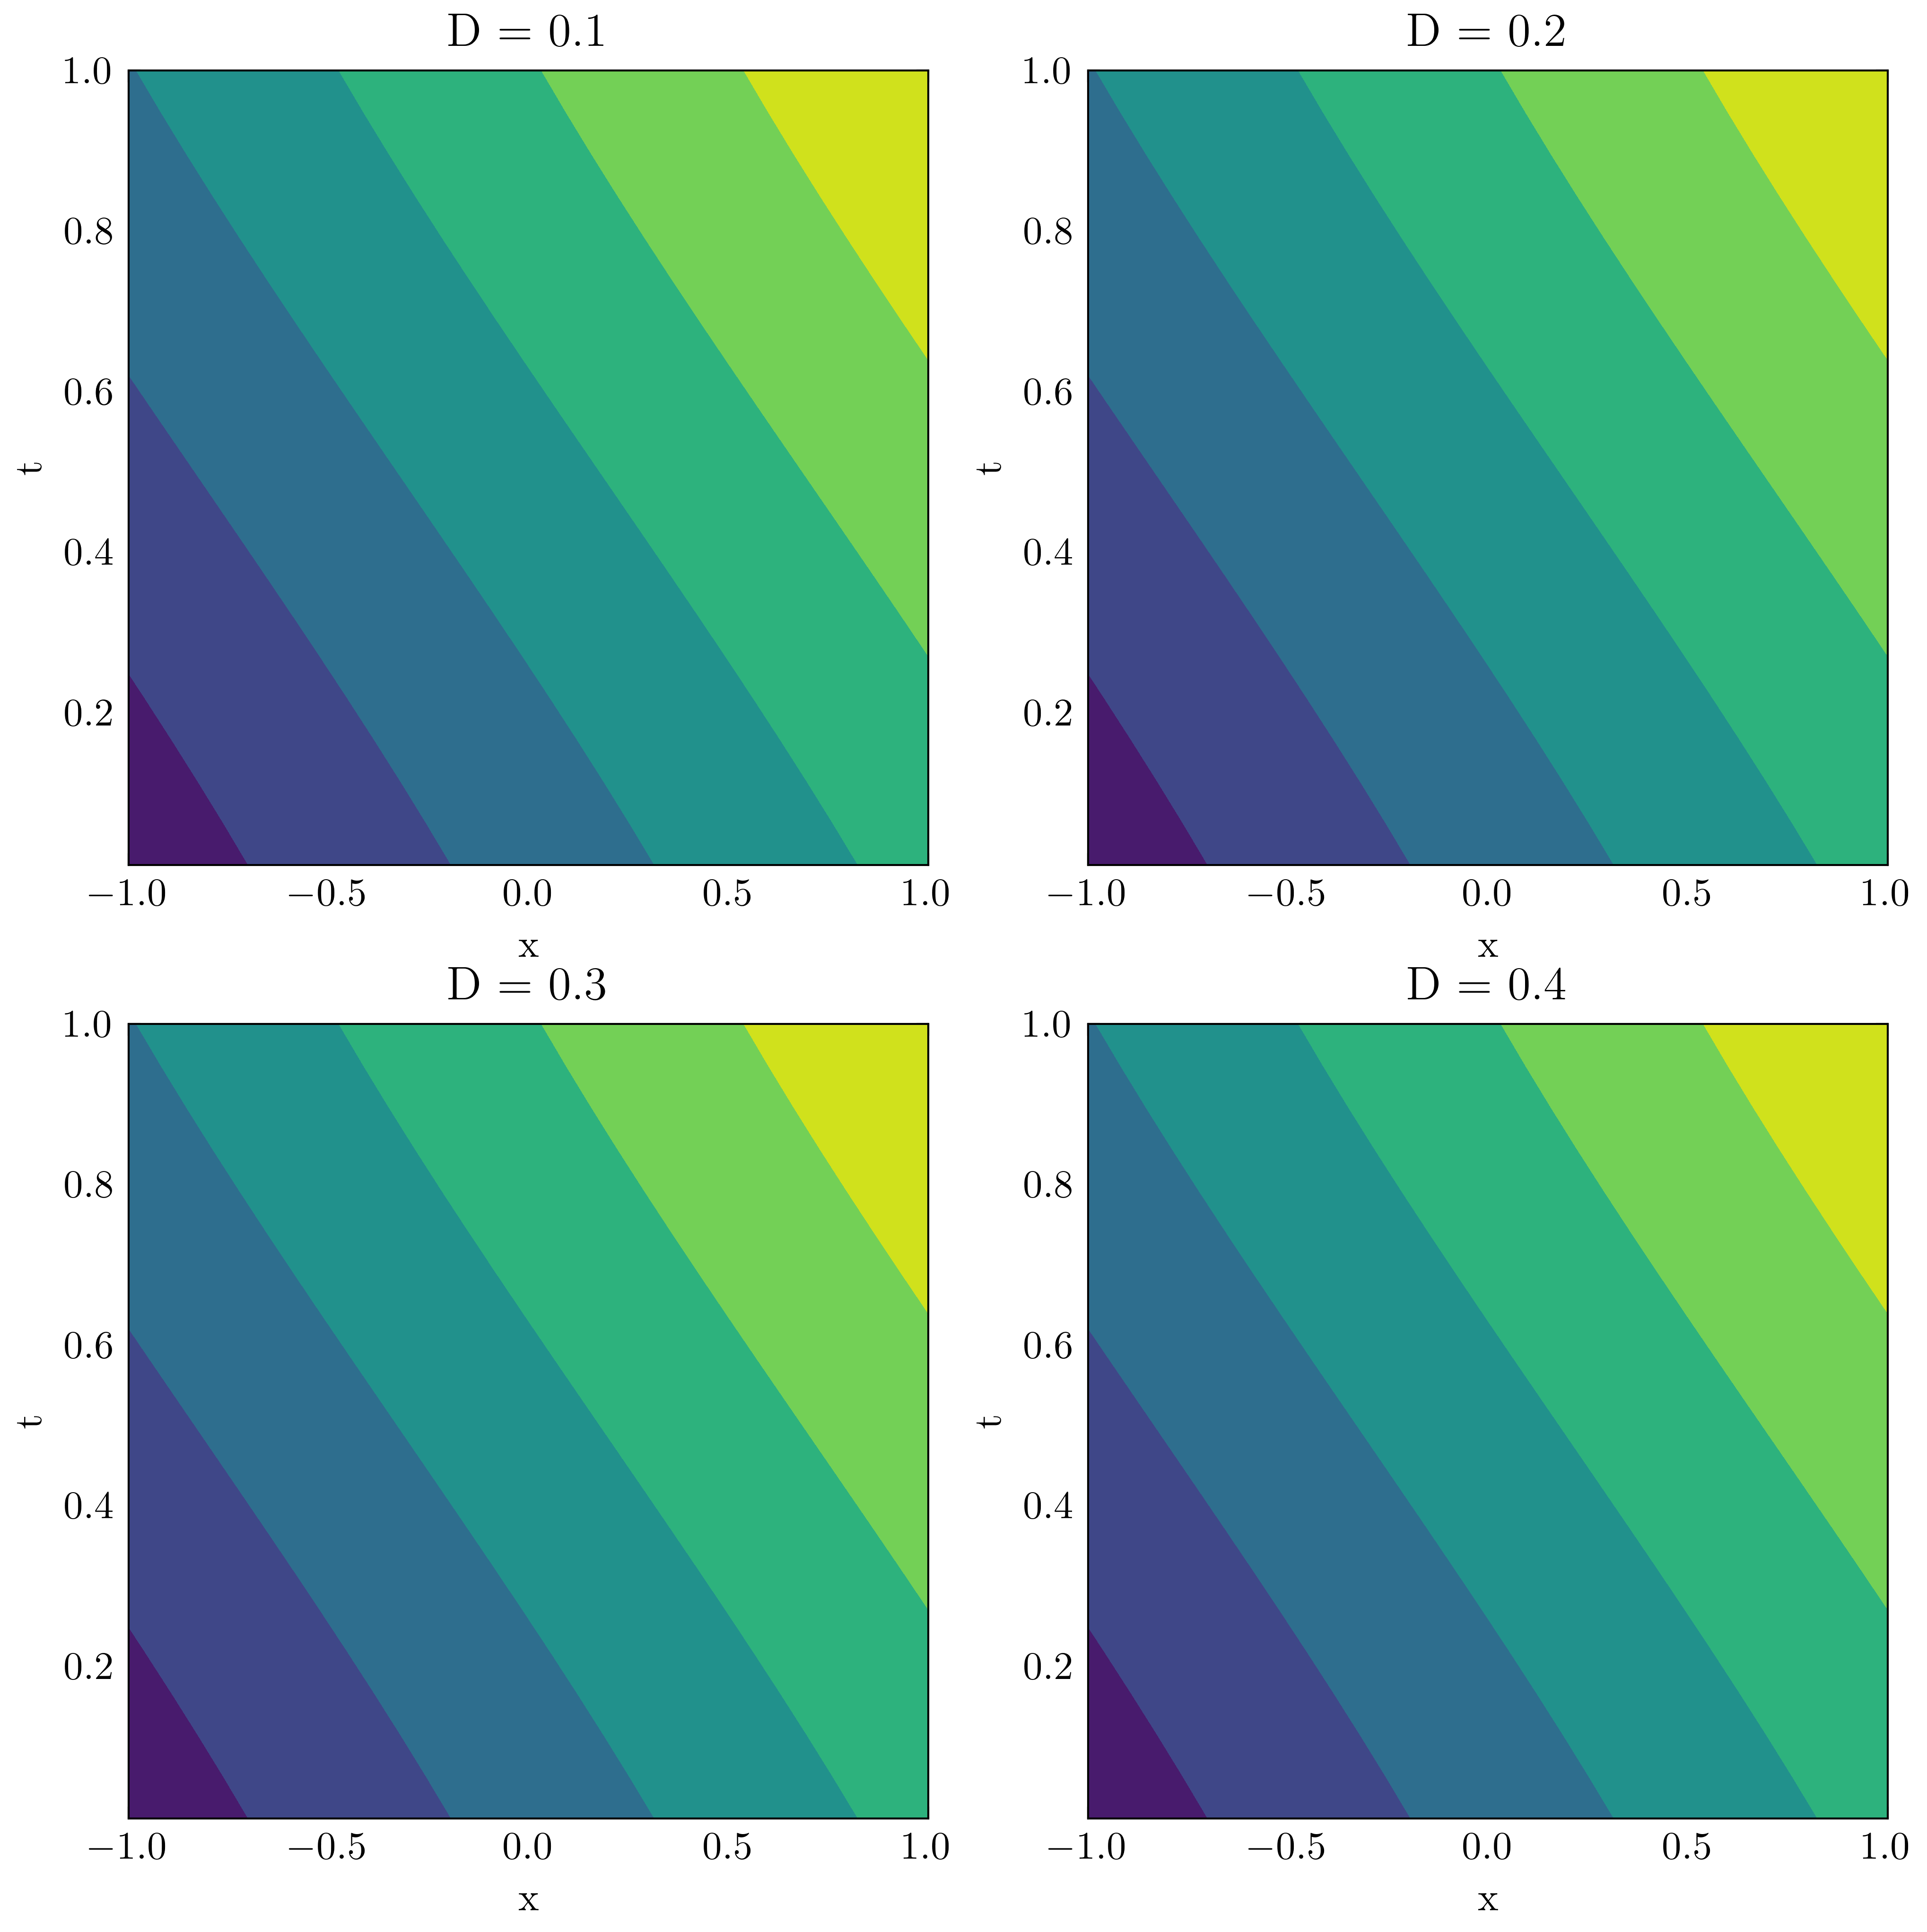
\includegraphics[width=.49\textwidth]{images/all.png}
\vspace*{-8mm}
\caption{Prediction values for four $D_1=0.1$, $D_2=0.2$, $D_3=0.3$, and $D_4=0.4$ coefficients}
\label{fig:alld}
\end{center}
\end{figure}

\subsection{Comparing Diffusion Across a Plate }
Another section of the code simulates the diffusion of heat through a two-dimensional square plate of size 10 mm x 10 mm with thermal diffusivity of water. The set up is similar except  diffusion of heat is governed by the heat equation, which describes how temperature changes over time in a given domain. The heat equation involves the second derivative of temperature with respect to both space and time. Thus, the plate has a circular region in the center with a high temperature and the rest of the plate is at a low temperature. Two graphs are generated using two different methods. The first section of the code (see Figure \ref{fig:cdm}) uses the forward-difference method in time and central-difference method in space to numerically solve the heat diffusion equation. The boundary conditions are set as cold on the bottom and sides and hot on top. The code outputs four figures at different timesteps that show the temperature distribution in the plate. 

The color scheme used in the maps represents temperature, with blue indicating the lowest temperature (273.15 K) and red indicating the highest temperature (373.15 K). The color scale is normalized to the initial and final temperatures of the plate, which are set to 273.15 K and 373.15 K, respectively. The temperature distribution on the plate can be observed by looking at the color distribution on the thermal maps.

Figure (\ref{fig:cnm}) on the other hand was generated by solving the heat diffusion equation using  the Crank-Nicolson method to calculate the next timestep of the temperature distribution. The temperature distribution is initialized with the initial temperature and then evolved in time with the specified boundary conditions until a final time as adapted from Arocha \cite{Arocha2018}. The temperature distribution at specific time intervals is saved and plotted the matplotlib library.

\begin{figure}[htb!]
\begin{center}
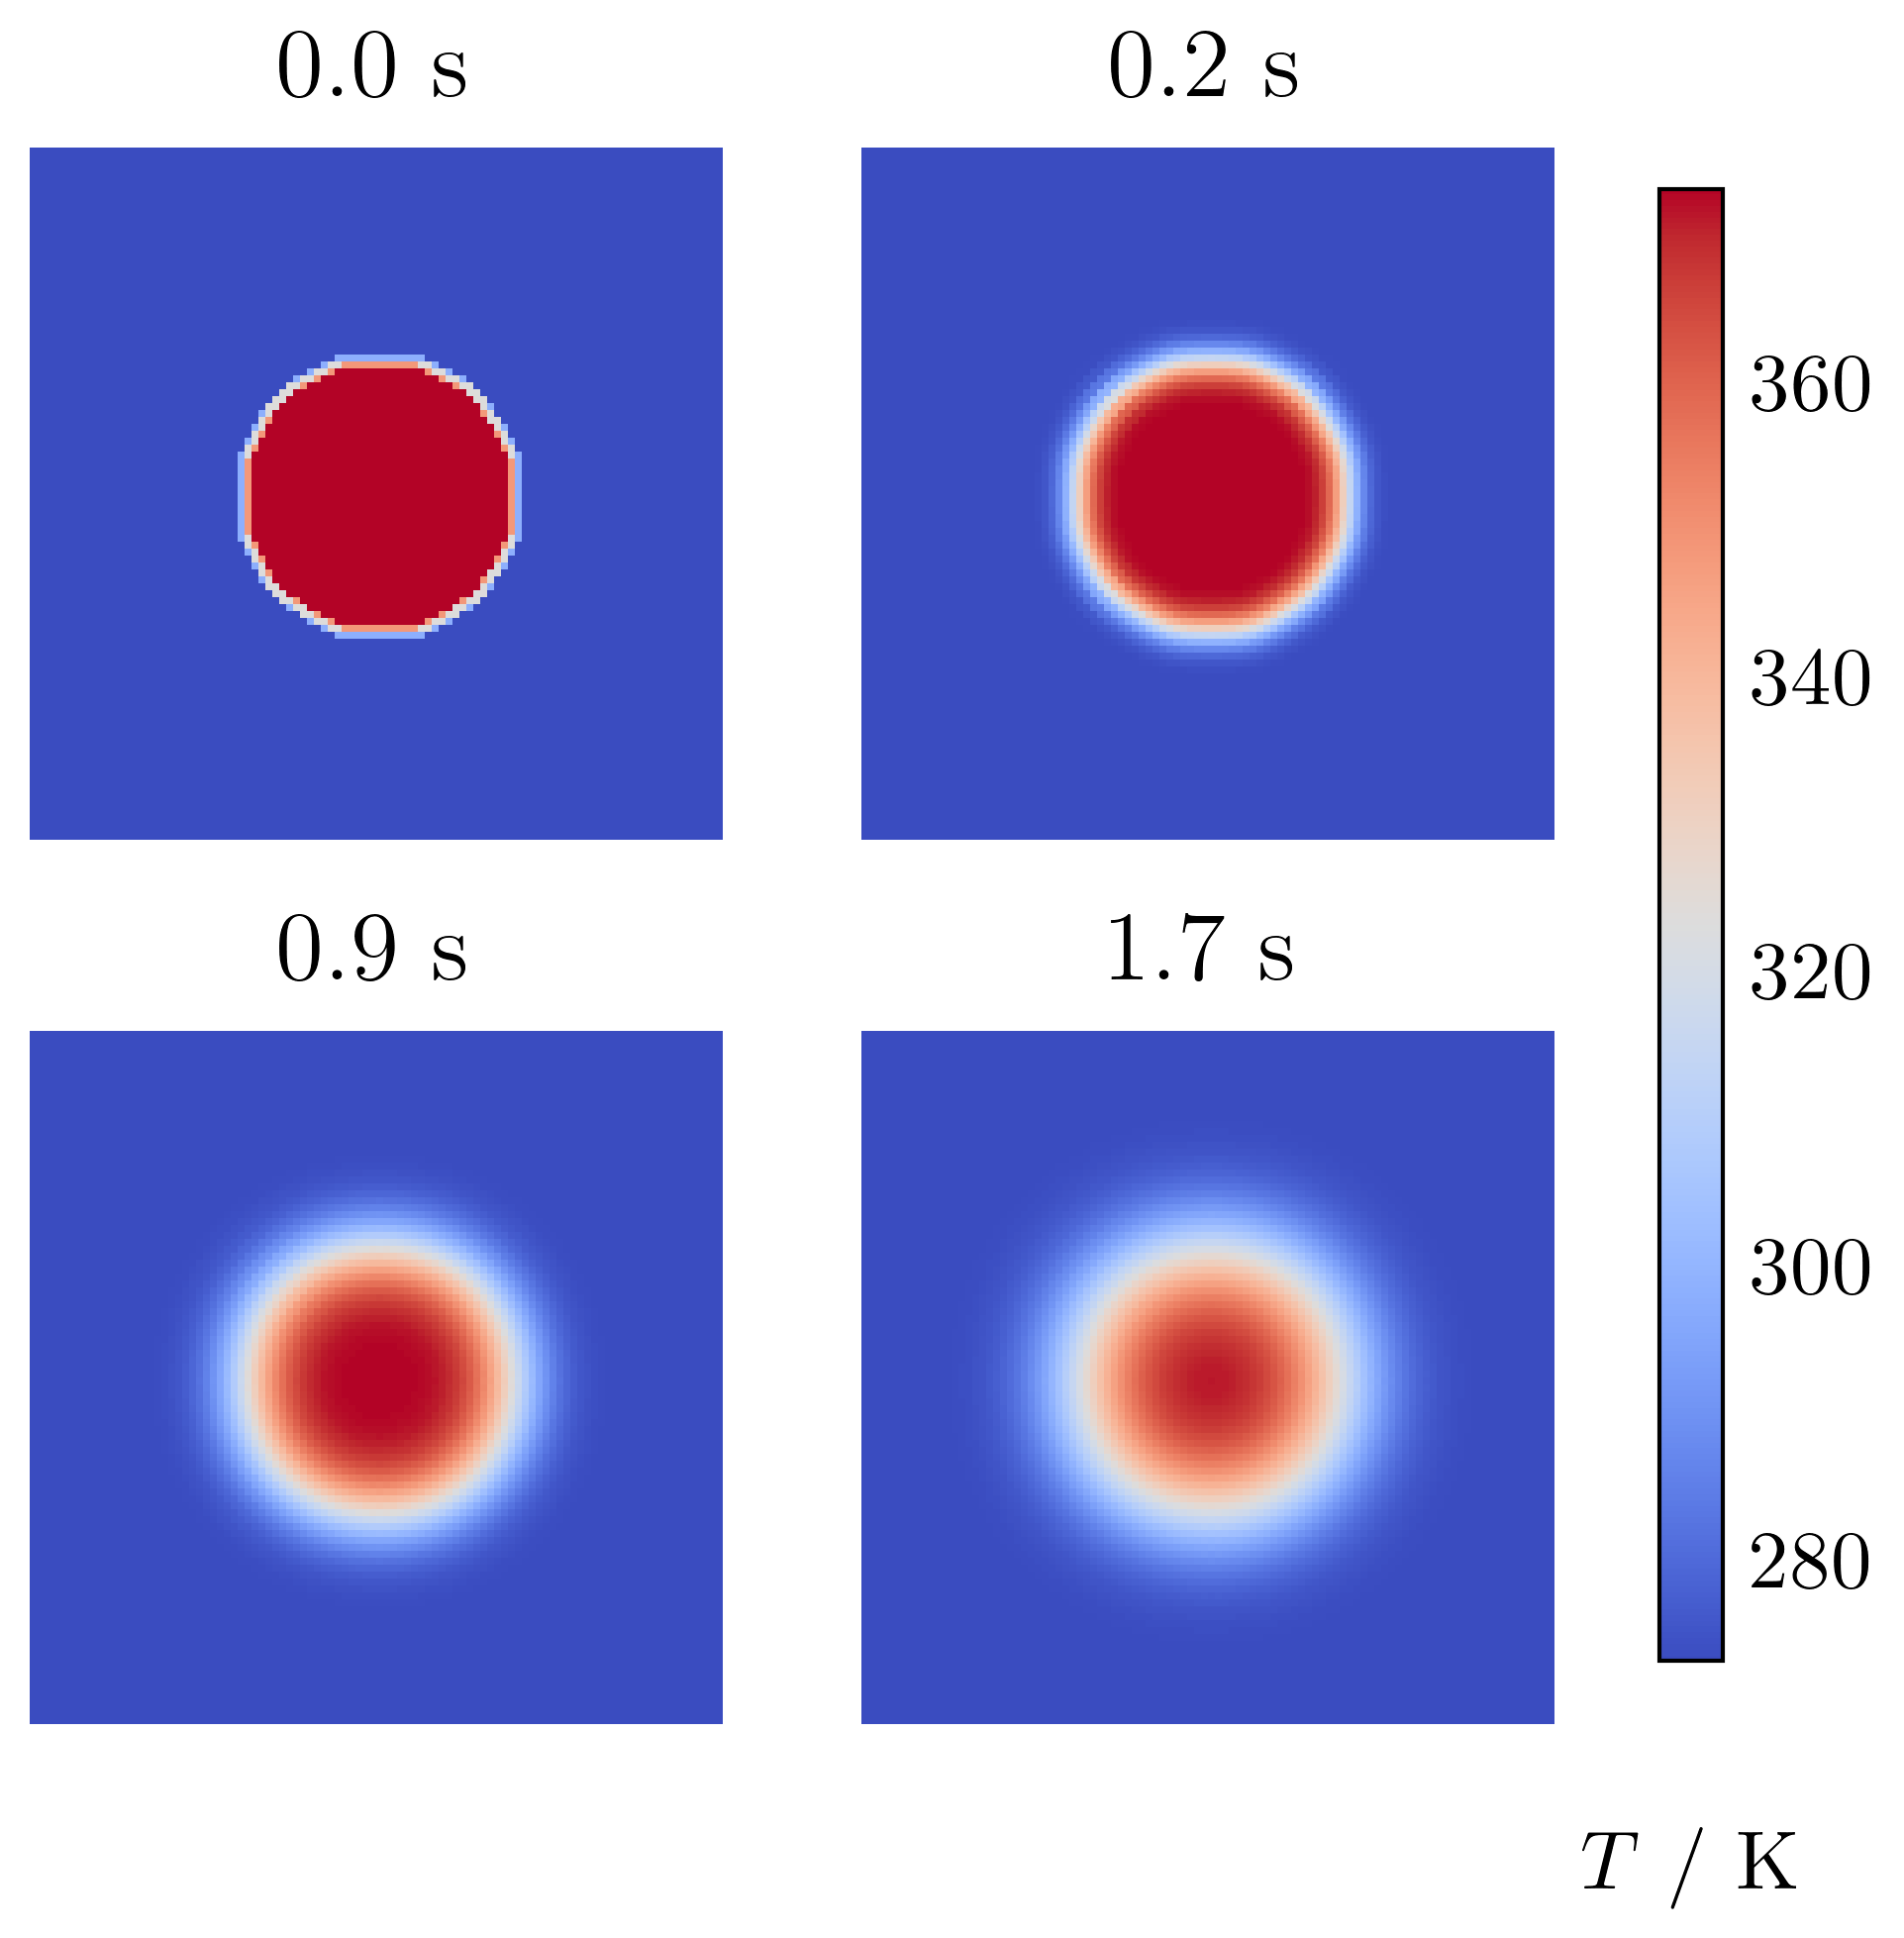
\includegraphics[width=.49\textwidth]{images/th_water.png}
\vspace*{-8mm}
\caption{Diffusion rate of water using forward-difference method in time and central-difference method in space. Normalized color scale to the initial and final temperatures of the plate, which are set to 273.15 K and 373.15 K, respectively based on the boundary conditions.}
\label{fig:cdm}
\end{center}
\end{figure}

\begin{figure}[htb!]
\begin{center}
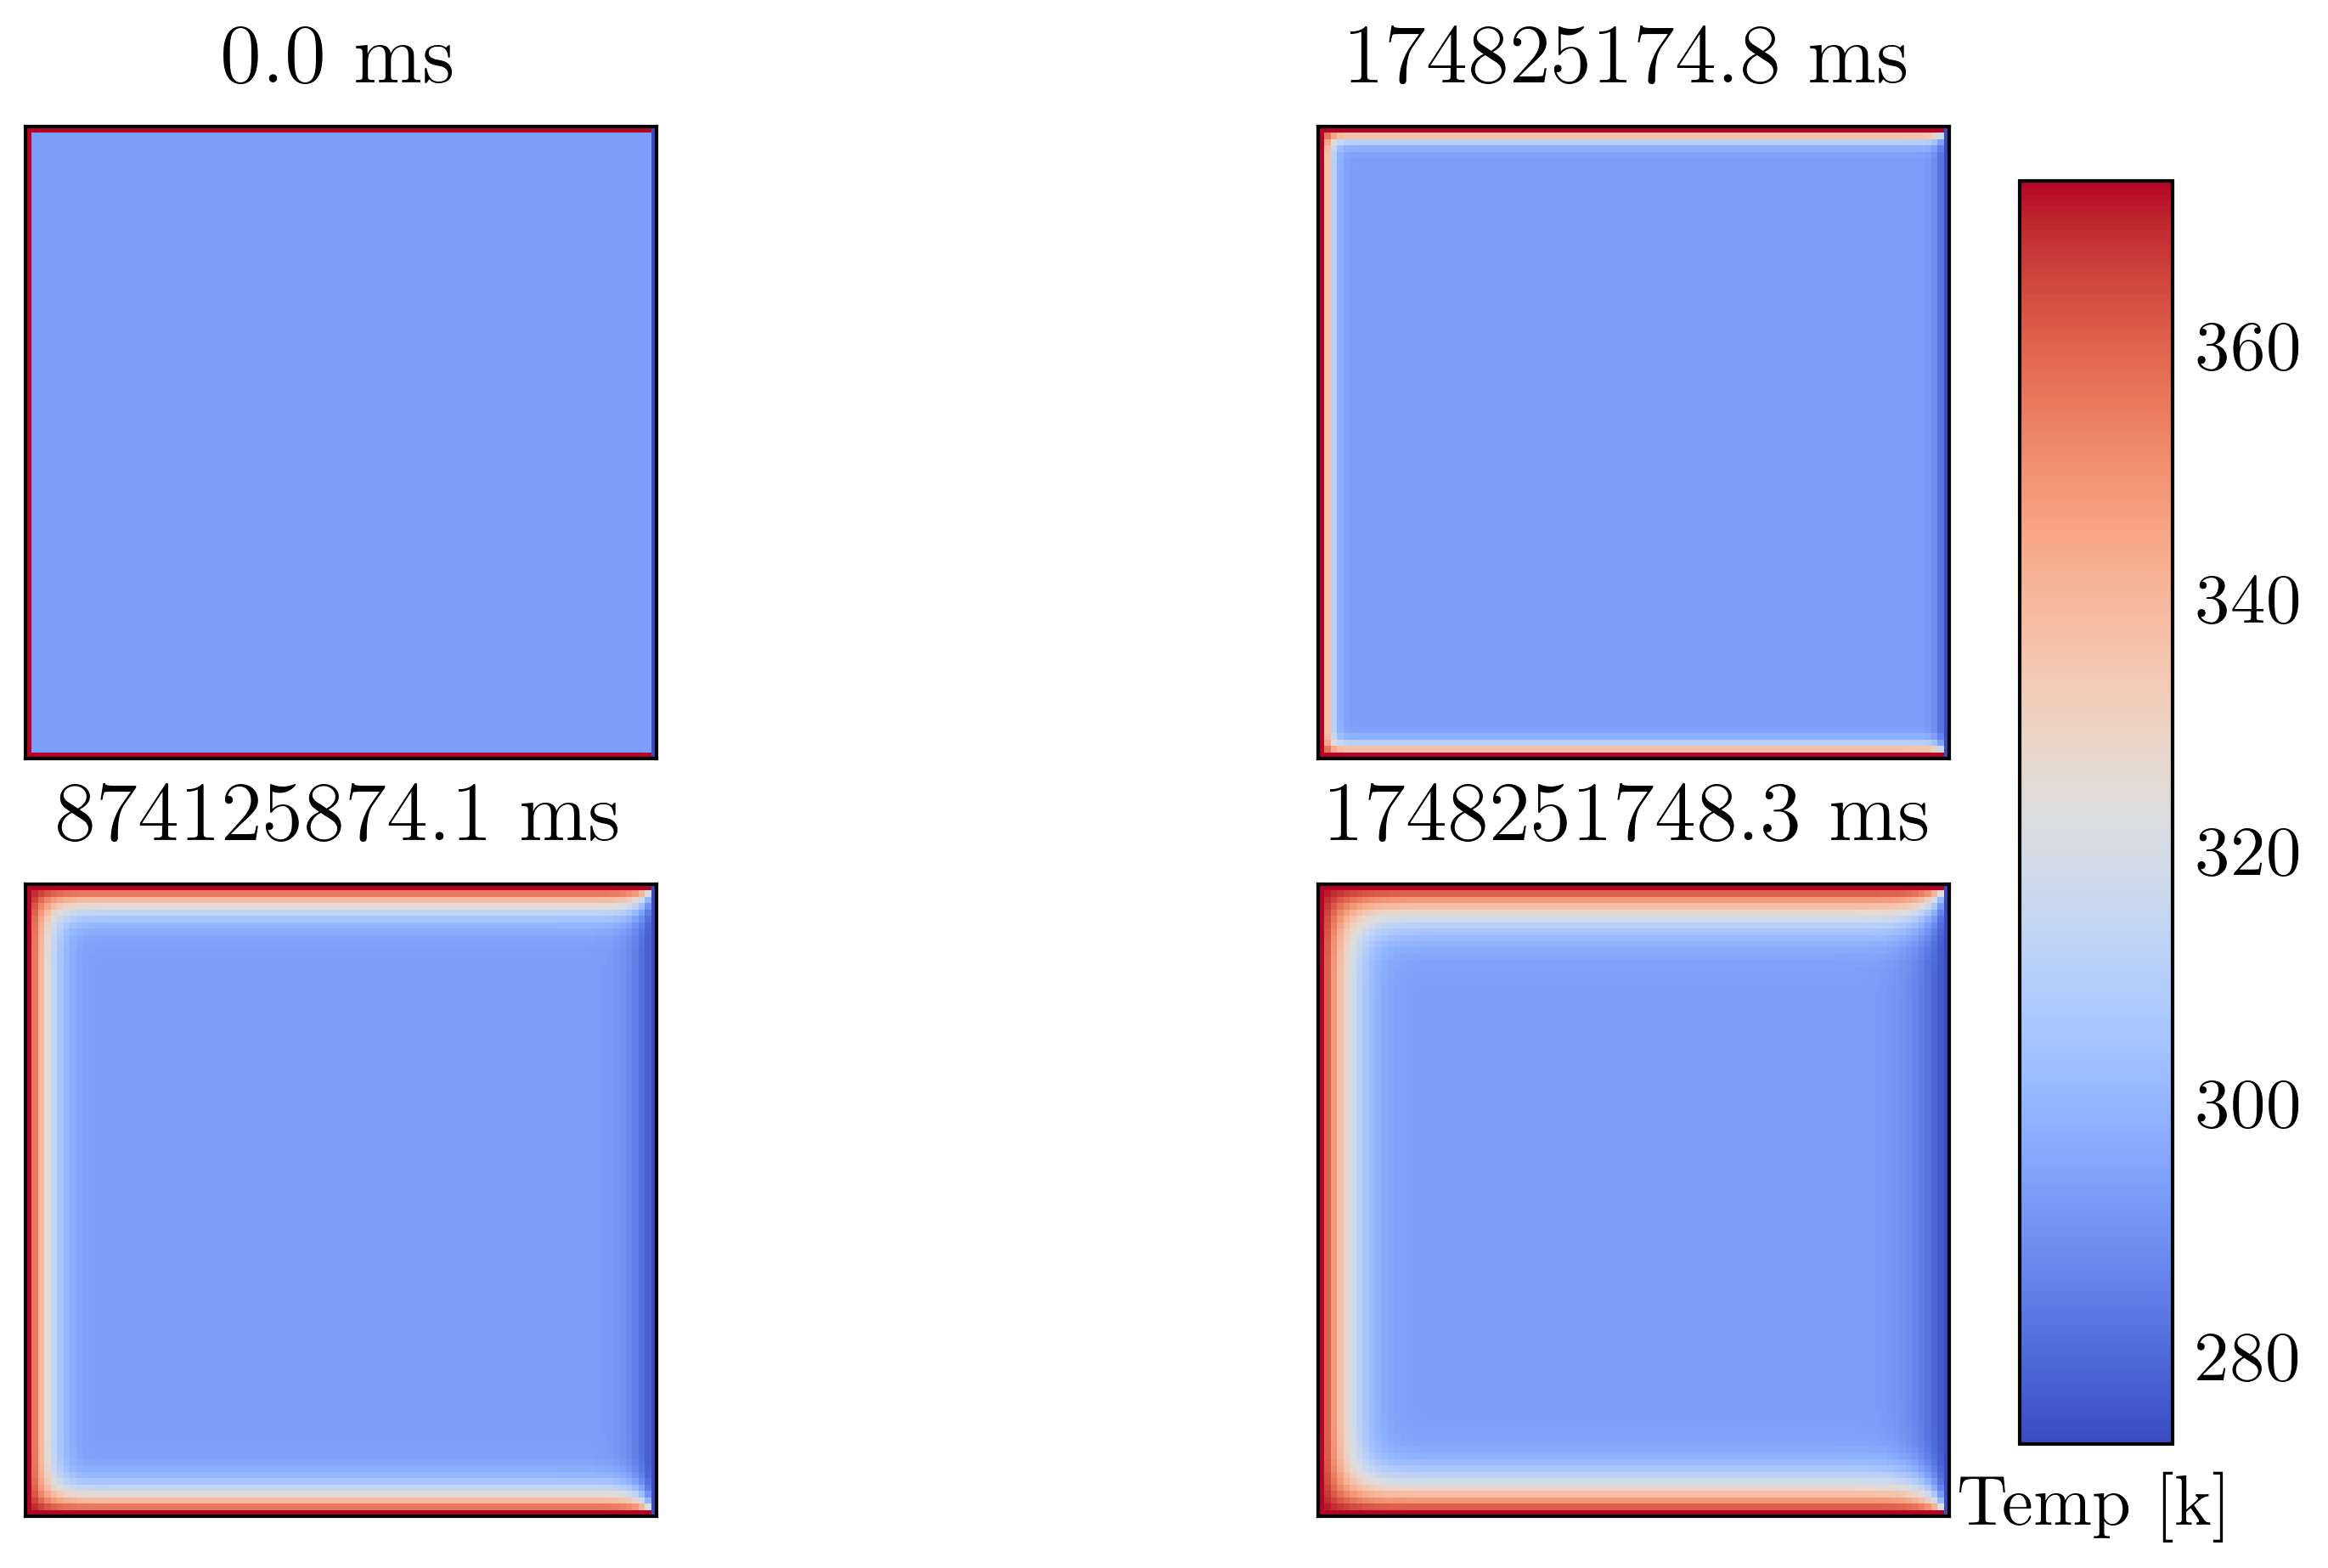
\includegraphics[width=.49\textwidth]{images/th_water_2.png}
\vspace*{-8mm}
\caption{Diffusion rate of water using Crank-Nicolson method, adapted from Arocha, 2018 \cite{Arocha2018} for comparison. The temperature distribution is initialized first and then evolved in continuous time with the specified boundary conditions until a certain value of time vector.}
\label{fig:cnm}
\end{center}
\end{figure}

Compared to the previous model, this one appears to be more specific to a particular physical system (heat diffusion in a plate of water), whereas the previous model was a general machine learning model that could be applied to various problems. Additionally, this model uses numerical methods to solve the differential equations governing the system, whereas the previous model did not explicitly solve differential equations. Both models have their own strengths and weaknesses and are applicable in different contexts.

\subsection{Using Finite Difference Method}
In Figure (\ref{fig:fdmm}) the code numerically solves a 2D diffusion equation with given boundary and initial conditions using the finite difference method. The final solution, represented by the array $U$, is then plotted using a heatmap with the matplotlib library. The resulting plot shows how the initial concentration profile evolves over time due to diffusion, with the red and blue colors representing high and low concentrations, respectively. 

\begin{figure}[htb!]
\begin{center}
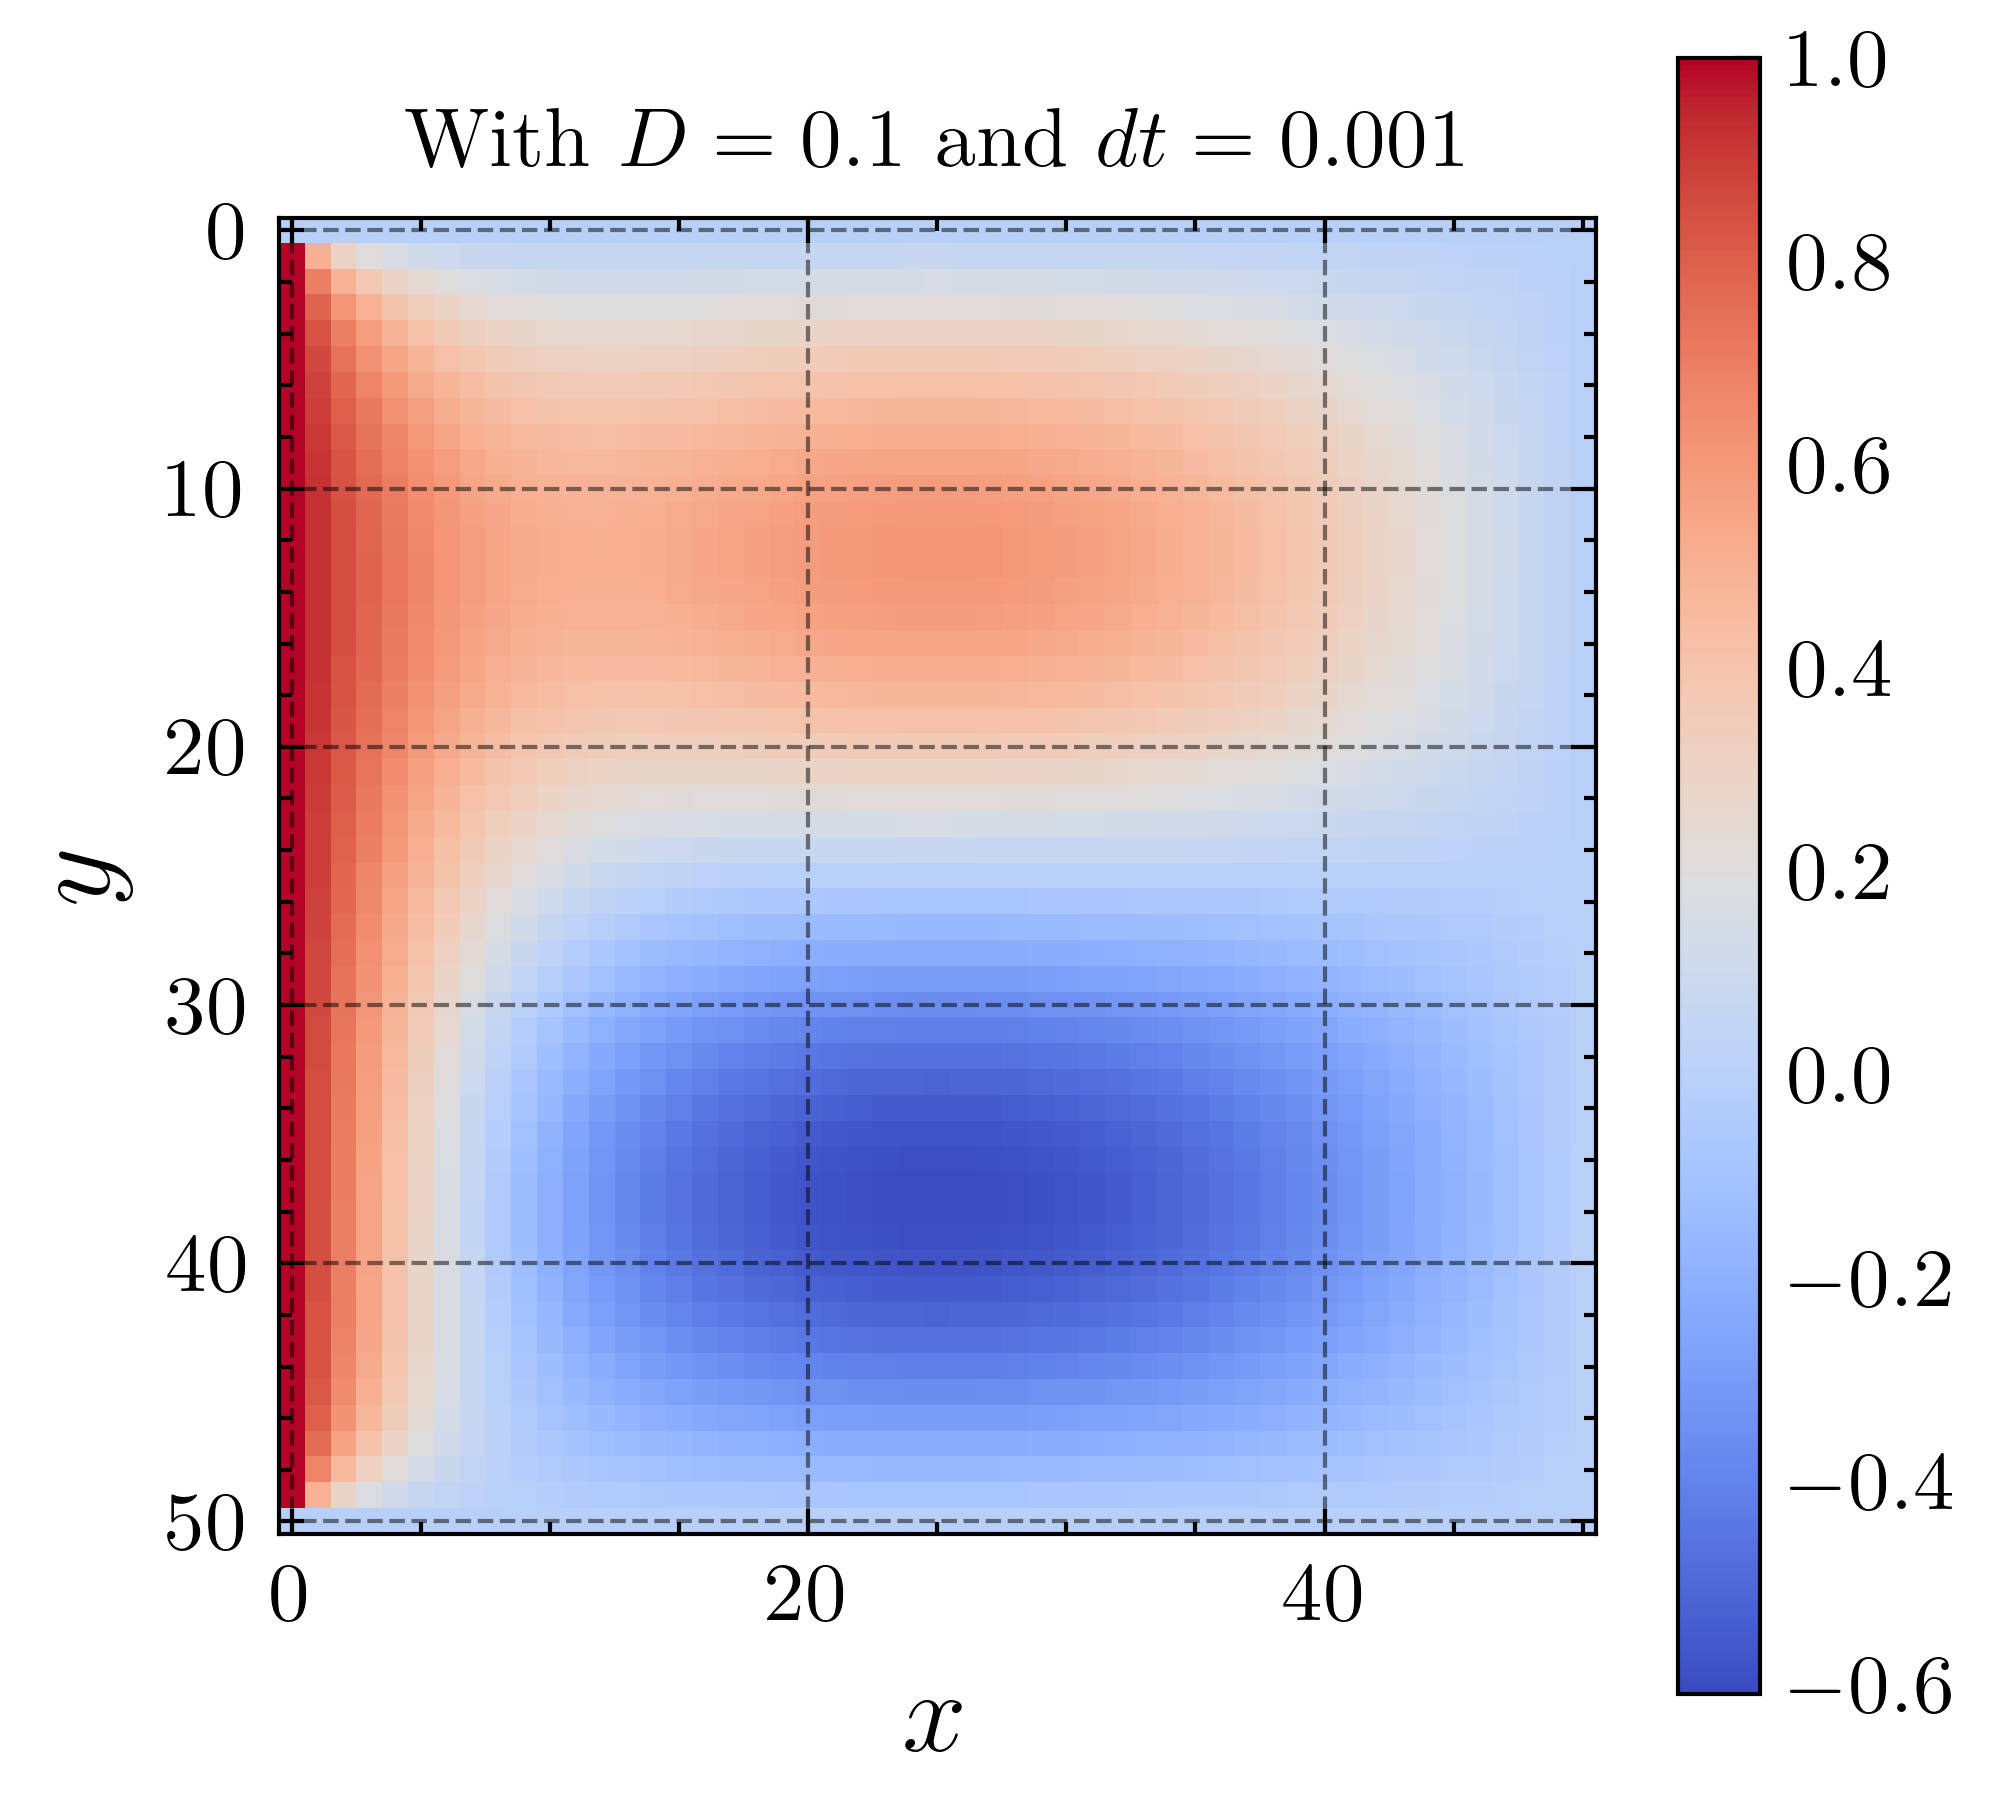
\includegraphics[width=.49\textwidth]{images/0.1_time.png}
\vspace*{-8mm}
\caption{D = 0.1 and T=0.001}
\label{fig:fdmm}
\end{center}
\end{figure}

This brief python code simulates the diffusion of a substance in a 2D domain. It defines the domain size and grid resolution, the diffusion coefficient, time step, and boundary conditions. It then creates the grid and initializes the solution array with the initial condition and boundary conditions. The code then iteratively computes the diffusion for each time step using a finite difference method and plots the final solution as shown above.

\subsection{Heat Flux and Temperature using Diffusion PiNN Model}

This section solves the two-dimensional diffusion equation using the PINN model provided in the code. The model is trained to predict the temperature distribution in the domain, given the diffusion coefficient and boundary conditions. The diffusion coefficient is defined as a function of the position, and four different values are used for comparison. The PINN model is defined with several dense layers and the loss function is defined as the mean square error between the predicted and actual temperature distributions. The model is trained using the RMSprop optimizer and the training data is generated by concatenating the $x$ and $y$ coordinates. The $x$ and $y $axes represent the spatial coordinates within the domain, and the colorbar on the right side of the plot indicates the temperature scale. Finally, the temperature distribution is plotted using for each diffusion coefficient. 

\begin{figure}[htb!]
\begin{center}
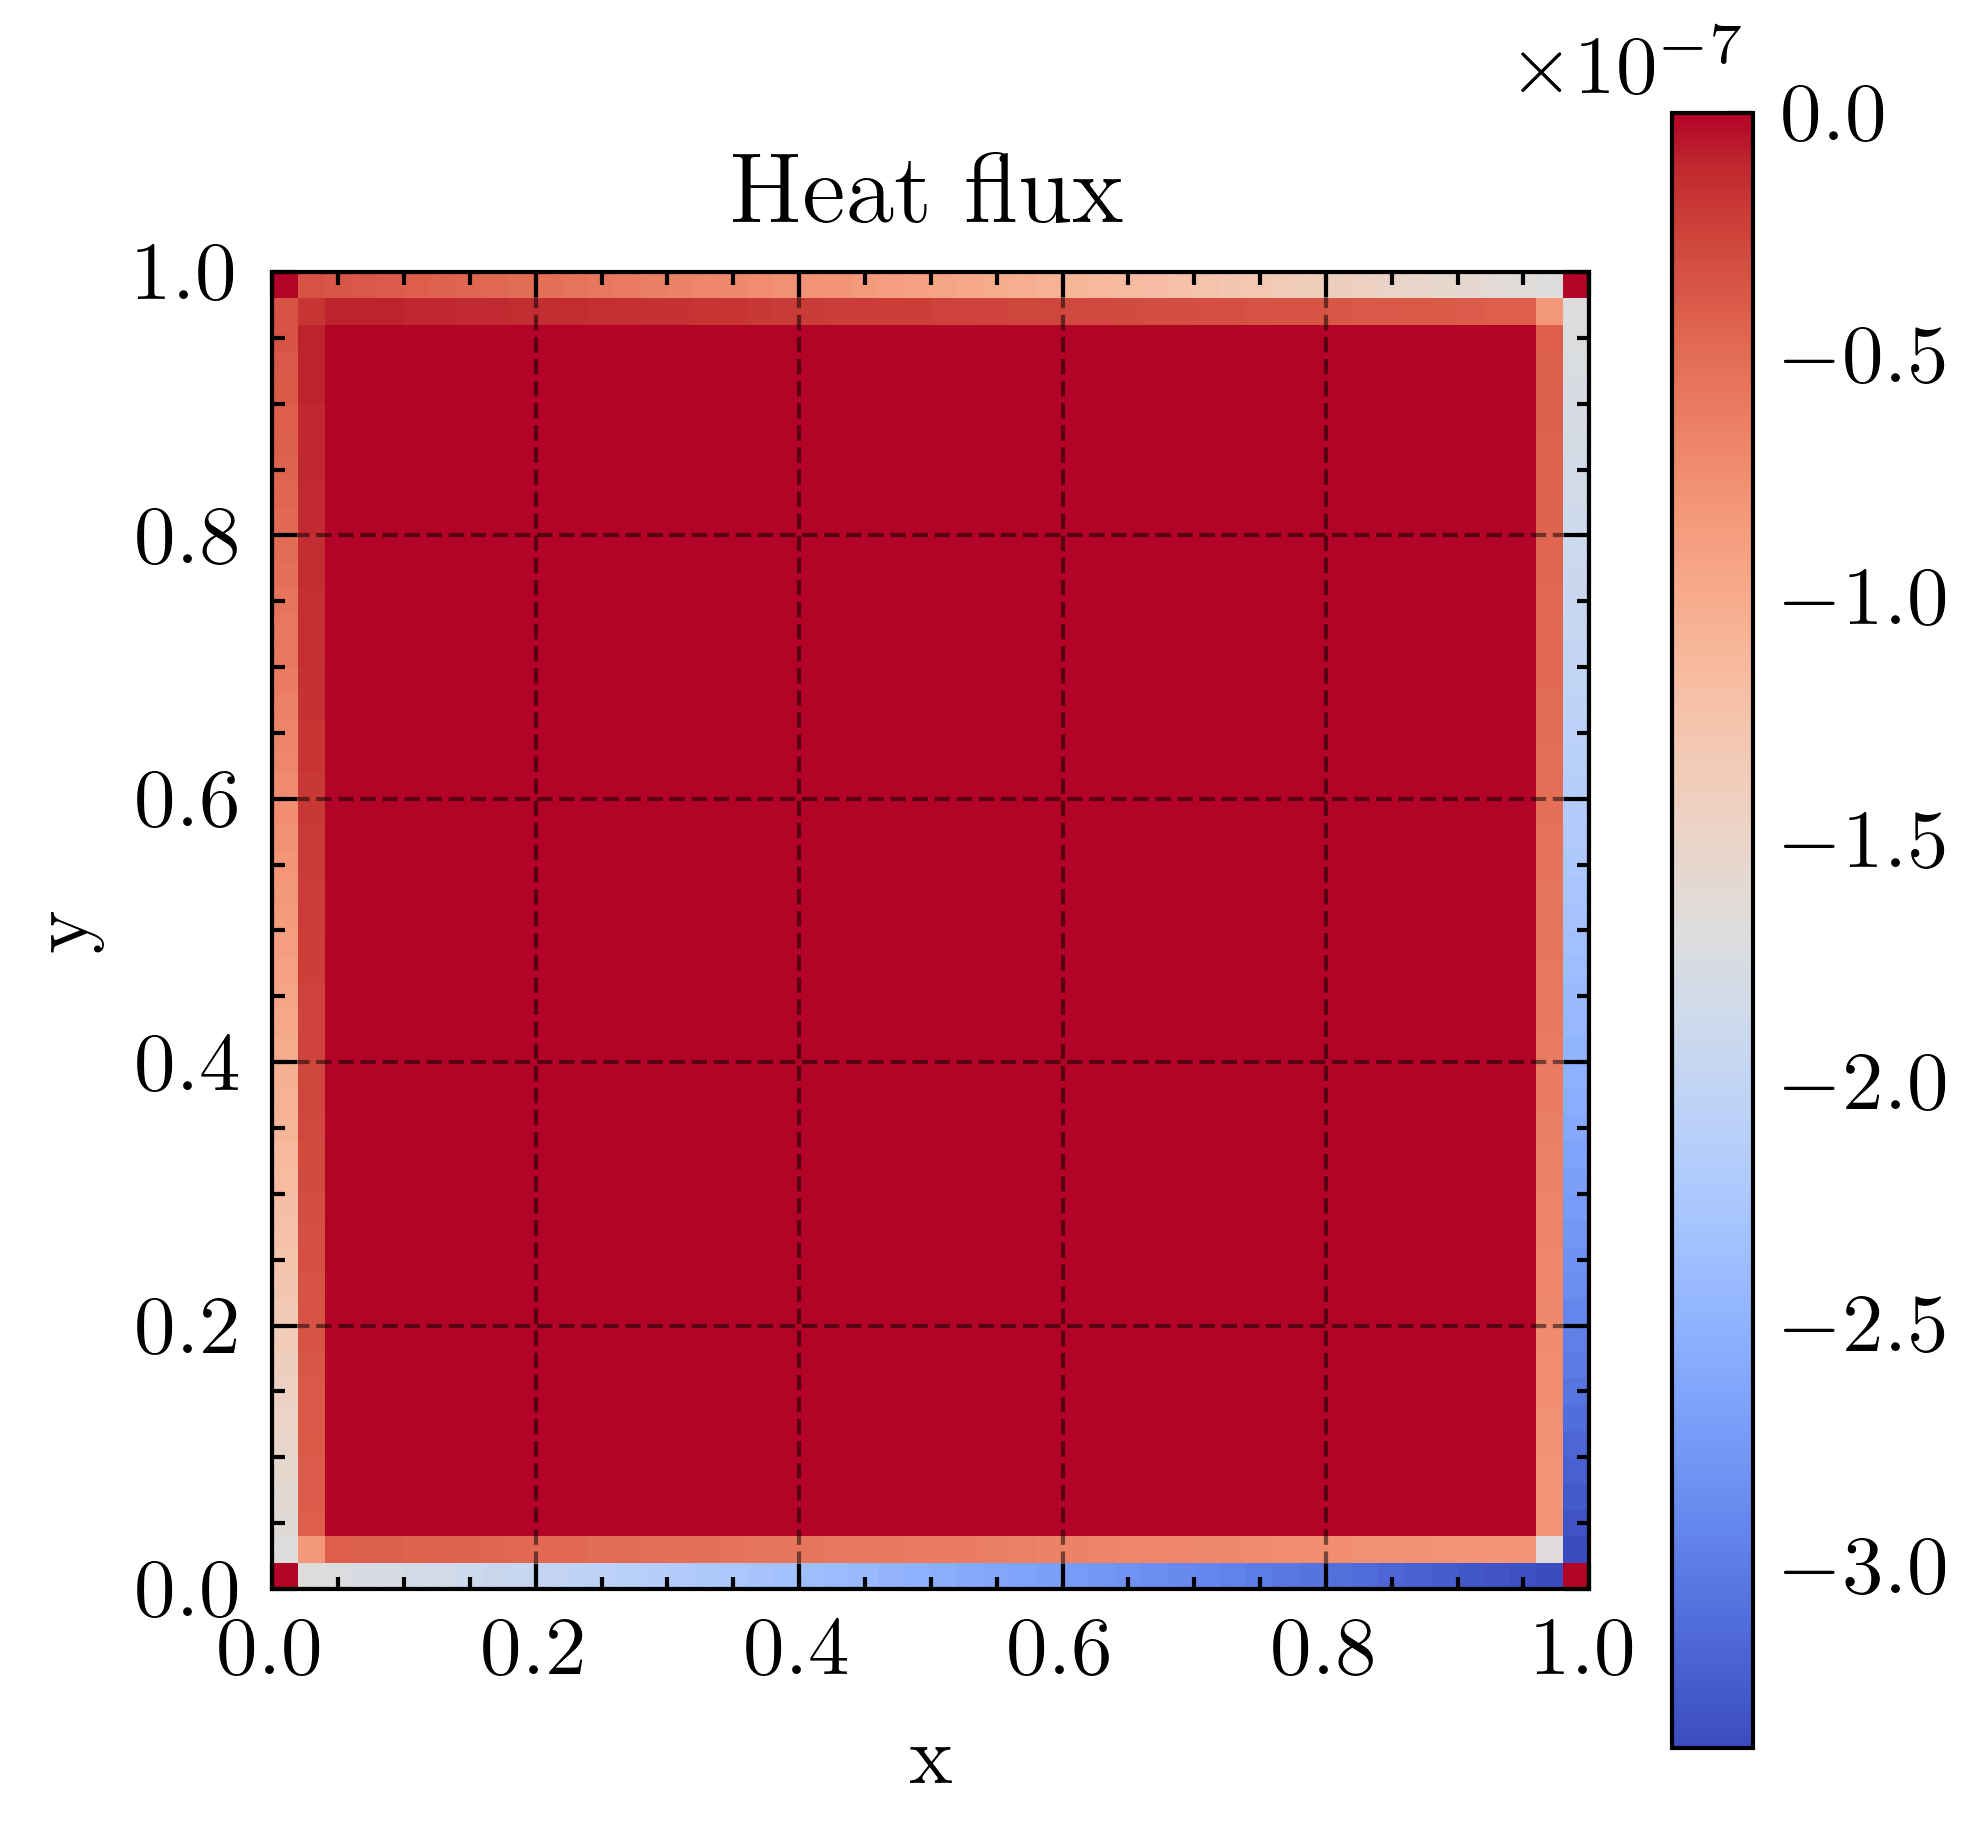
\includegraphics[width=.49\textwidth]{images/heat_flux.png}
\vspace*{-8mm}
\caption{Heat Flux as the gradient of the temperature distribution. A positive value indicates heat flowing in the positive $+x$ or $+y$ direction, while a negative value indicates heat flowing in the negative $-x$ or $-y$ direction}
\label{fig:hf}
\end{center}
\end{figure}

The heat flux plot (Figure (\ref{fig:hf})) shows the rate of heat transfer per unit area in the system. In this case, the heat flux is calculated as the gradient of the temperature distribution. Positive values of the heat flux indicate heat flowing in the positive $x$ or $y$ direction, while negative values indicate heat flowing in the negative $x$ or $y$ direction. The heat flux plot can provide additional insights into the behavior of the system, such as identifying regions of high or low heat transfer and the direction of heat flow.

\begin{figure}[htb!]
\begin{center}
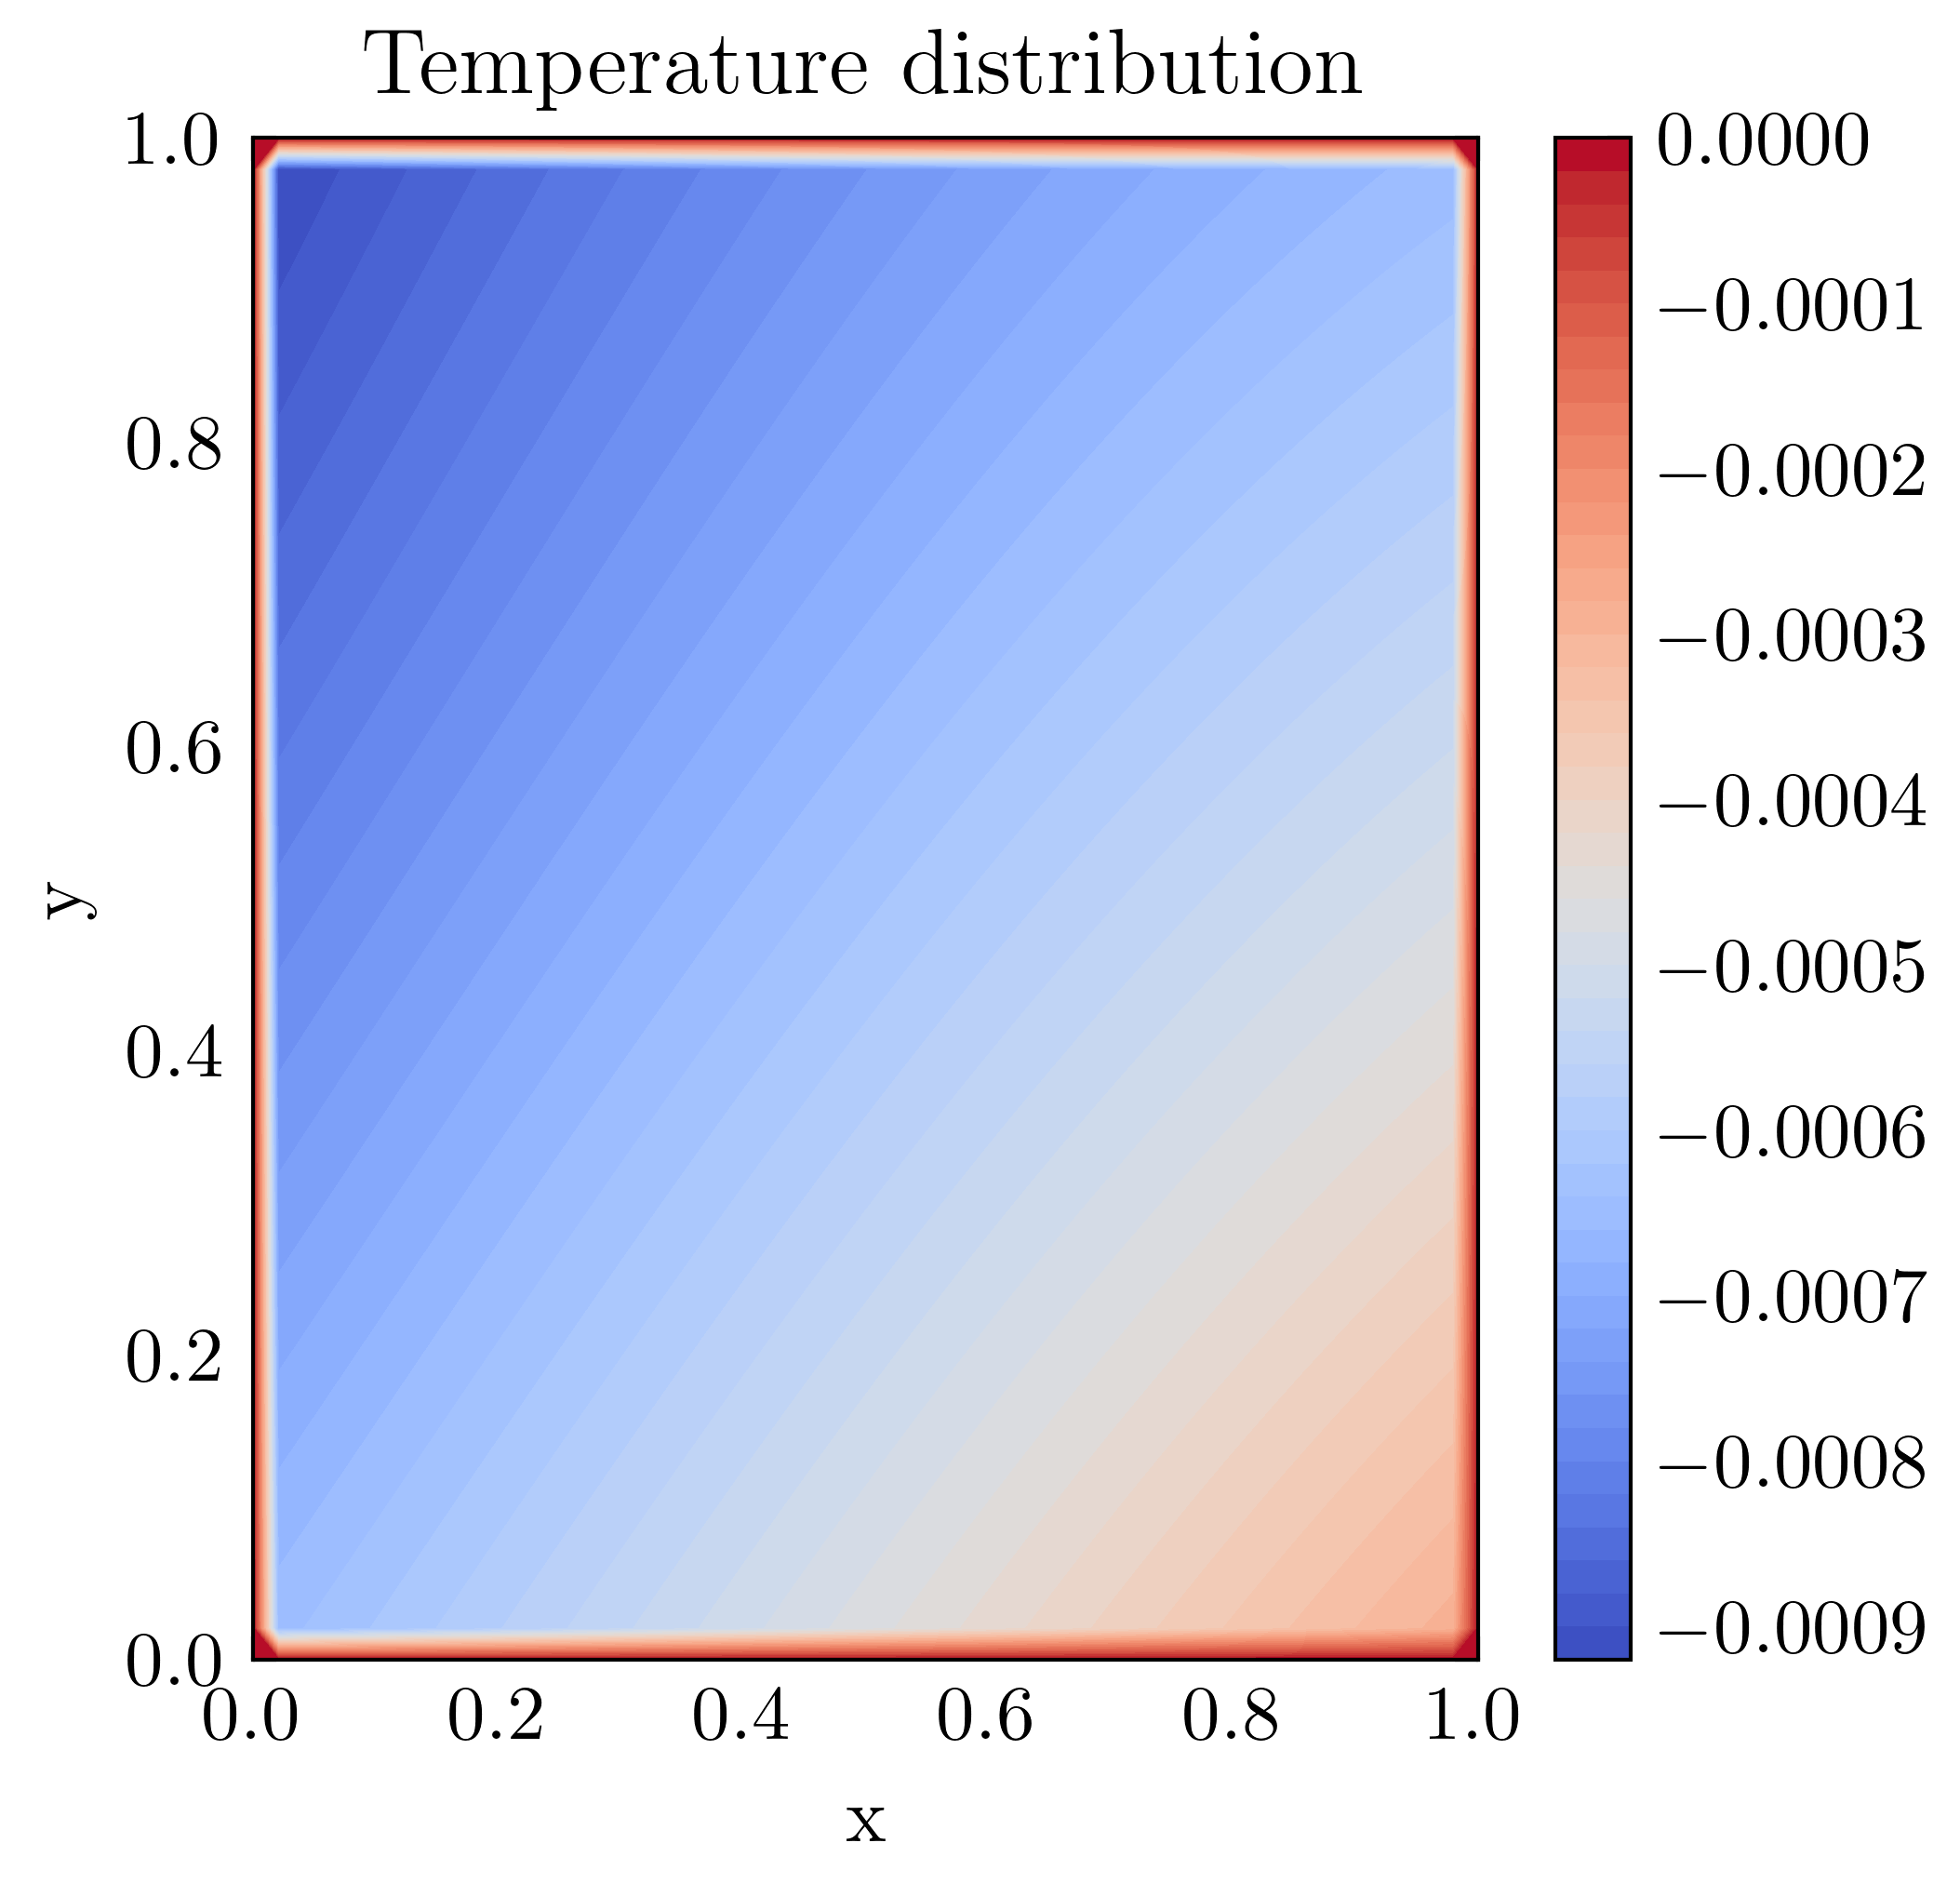
\includegraphics[width=.49\textwidth]{images/temp_dist.png}
\vspace*{-8mm}
\caption{Temperature distribution, across the various $x$ and $y$ values in the plate. Red corresponds to high temperatures while blue corresponds to values at low temperatures}
\label{fig:tmd}
\end{center}
\end{figure}

In a different section of the code, the Dirichlet boundary condition \cite{Sukumar2022}  was used was; where the temperature is specified on the boundaries of the domain. Specifically, the temperature is set to zero on the top, bottom, left, and right boundaries of the square domain. Figure (\ref{fig:tmd}) shows the temperature distribution across the various $x$ and $y$ values in the plate. The color of the plot represents the temperature distribution, where red corresponds to high temperatures and blue corresponds to low temperatures. And finally, the heat map plot in Figure (\ref{fig:t01}) shows the circular cross-sectional temperature profile at time = 1 second, providing a color heat map of the similar scale.  

\begin{figure}[htb!]
\begin{center}
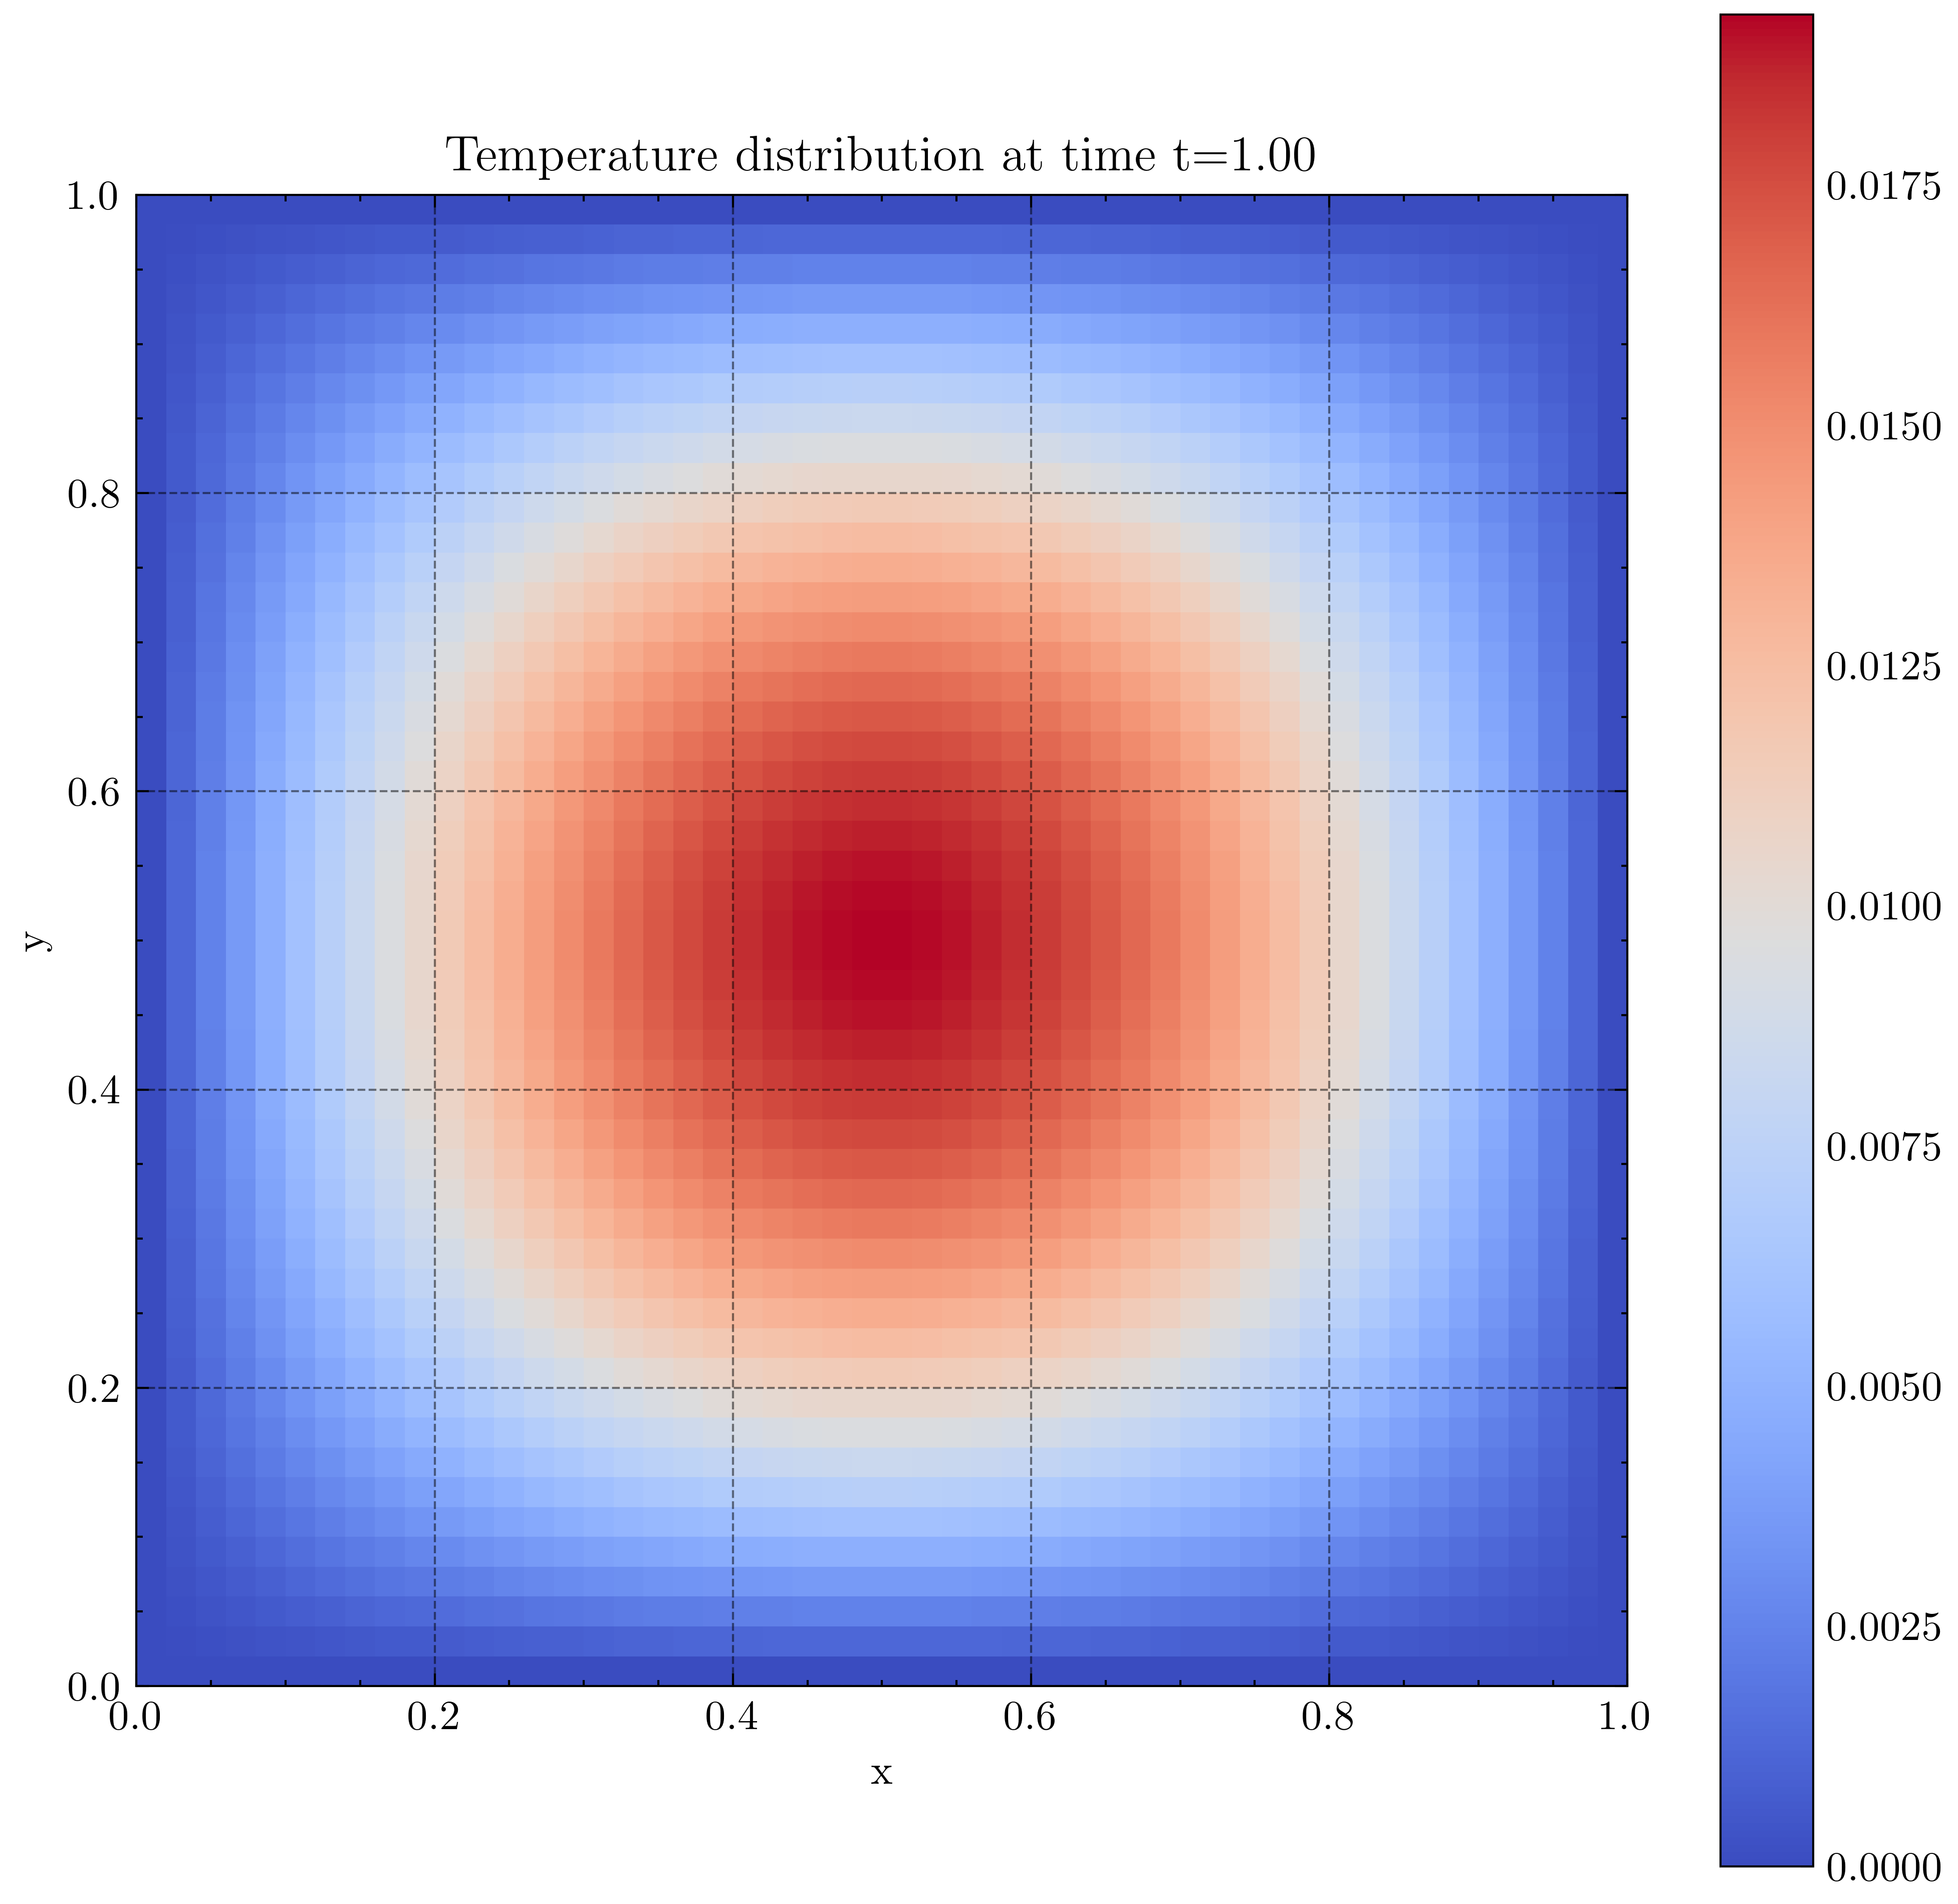
\includegraphics[width=.49\textwidth]{images/teemp_dist_time.png}
\vspace*{-8mm}
\caption{Heat map for a circular cross-section of temperature Profile at $Time = 1$ seconds}
\label{fig:t01}
\end{center}
\end{figure}

